%%% Local Variables:
%%% coding: utf-8
%%% mode: latex
%%% TeX-engine: xetex
%%% End:
\documentclass[10pt]{beamer}
% NOTE May need to manually set tex engine in emacs

\usetheme[progressbar=frametitle]{metropolis}
\usepackage{appendixnumberbeamer}

\usepackage{svg}
\usepackage{ulem}
\usepackage{cancel}

\usepackage{pifont}
\newcommand{\cmark}{\ding{51}}
\newcommand{\xmark}{\ding{55}}

\usepackage[dvipsnames]{xcolor}
\definecolor{mLightGreen}{HTML}{14B03D}

\usepackage{booktabs}
\usepackage[scale=2]{ccicons}

\usepackage{graphicx}

\usepackage{pgfplots}
\usepgfplotslibrary{dateplot}

\usepackage{todonotes}
\newif\ifdraft
\drafttrue
\newcommand{\todoin}[1]{\ifdraft{\todo[inline]{TODO:\@ #1}}\fi}

\usepackage{xspace}
\usepackage{mathpartir}
\newcommand{\themename}{\textbf{\textsc{metropolis}}\xspace}

\newcommand{\Set}{\mathbf{Set}}
\newcommand{\String}{\mathbf{String}}
\newcommand{\simulsubst}[2]{#1\{#2\}}
\newcommand{\subst}[3]{\simulsubst {#1} {#2/#3}}
\newcommand{\letin}[3]{\mathsf{let}\, #1 = #2 \, \mathsf{in}\, #3}
\newcommand{\lamb}[2]{\lambda #1.\, #2}
\newcommand{\lamblto}[2]{\lambda^{{\lto}} #1.\, #2}
\newcommand{\lambtol}[2]{\lambda^{{\tol}} #1.\, #2}
\newcommand{\dlamb}[2]{\overline{\lambda} #1.\, #2}
\newcommand{\app}[2]{#1 \, #2}
\newcommand{\applto}[2]{#1 \mathop{{}^{\lto}} #2}
\newcommand{\apptol}[2]{#1 \mathop{{}^{\tol}} #2}
\newcommand{\PiTy}[3]{\Pi #1 : #2.\, #3}
\newcommand{\SigTy}[3]{\Sigma #1 : #2.\, #3}
\newcommand{\LinPiTy}[3]{\widebar\Pi #1 : #2.\, #3}
\newcommand{\LinSigTy}[3]{\widebar\Sigma #1 : #2.\, #3}
\newcommand{\amp}{\mathrel{\&}}
\newcommand{\GrTy}{\mathsf{Gr}}

\newcommand{\ctxwff}[1]{#1 \,\, \mathsf{ok}}
\newcommand{\ctxwffjdg}[2]{#1 \vdash #2 \,\, \mathsf{type}}
\newcommand{\linctxwff}[2]{#1 \vdash #2 \,\, \mathsf{ok}}
\newcommand{\linctxwffjdg}[2]{#1 \vdash #2 \,\, \mathsf{linear}}

\usetikzlibrary{automata, positioning, arrows, fit}
\usetikzlibrary{shapes,arrows,calc,positioning,trees}
\tikzset{
  invisible/.style={opacity=0},
  visible on/.style={alt={#1{}{invisible}}},
  alt/.code args={<#1>#2#3}{%
    \alt<#1>{\pgfkeysalso{#2}}{\pgfkeysalso{#3}} % \pgfkeysalso doesn't change the path
  },
}
\usepackage{jigsaw}


\title{\large Formal Grammars as Types in Non-commutative Linear-non-linear Type Theory}
\date{\today}
\author{Steven Schaefer}
\institute{University of Michigan}
% \titlegraphic{\includegraphics[height=1.5cm]{figures/umich.png}}
%

% \usepackage[backend=bibtex]{biblatex}
% \addbibresource{refs}
%
\AtBeginSection{
\begin{frame}
  \setbeamertemplate{section in toc}[sections numbered]
  \tableofcontents[currentsection]
\end{frame}
}

\begin{document}

\maketitle

\metroset{block=fill}

\section{Introduction}

\begin{frame}
  \setbeamertemplate{section in toc}[sections numbered]
  \tableofcontents[currentsection]
\end{frame}

\begin{frame}{Parsing is Everywhere}
  A \emph{parser} emits structured data from an input string

  \onslide<2->{
  \begin{center}
  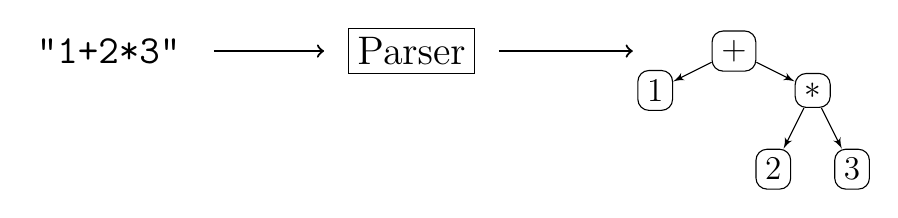
\begin{tikzpicture}[
    treenode/.style = {shape=rectangle, rounded corners,
    draw, align=center, font=\large,
    top color=white, bottom color=white!20},
    line/.style={draw, -latex'},
    edge from parent/.style={draw,-latex'},
    level 1/.style={sibling distance=20mm, level distance=0.5cm},
    level 2/.style={sibling distance=1cm, level distance=1cm}]

    \node (src) {\Large \texttt{"1+2*3"}};

    \node[right=2cm of src, shape=rectangle, draw] (parser) {\Large Parser};

    \node[right=3cm of parser, treenode] (tree) {$+$}
    child { node[treenode] (one) {$1$} }
    child { node[treenode] (times){$\ast$}
        child { node[treenode] {$2$} }
        child { node[treenode] {$3$} }
      };


  \draw [->, thick, shorten <= 0.3cm, shorten >= 0.3cm] (src) -- (parser);
  \draw [->, thick, shorten <= 0.3cm, shorten >= 1cm] (parser) -- (tree);

  \end{tikzpicture}
  \end{center}
  }

  \onslide<3->{
  Ubiquitous in computer science,
  \begin{itemize}
    \item<4-> Data serialization
    \item<5-> Natural language processing
    \item<6-> \textbf{Programming language implementation}
      \begin{itemize}
        \item<7-> High-level source code must be understood by the machine
        \item<8-> Translation from user-written code to an abstract syntax tree (AST)
      \end{itemize}
  \end{itemize}
  }

\end{frame}

% \begin{frame}{Compilers: Do They Work?}
%   \begin{center}
%   \begin{tikzpicture}[node distance=3.7cm]
%     \node (sourceCode) [visible on=<2->] {\includegraphics[width=2cm]{figures/srccode.png}};
%     \node (srcLabel) [above=-0.3cm of sourceCode,visible on=<2->] {Source Code};
%     \node (compiler) [right of=sourceCode, visible on=<1->] {\includegraphics[width=1cm]{figures/c.png}};
%     \node (compilerLabel) [above=-0.3cm of compiler, visible on=<1->] {C Compiler};
%     \node (outputCode) [right of=compiler, visible on=<3->] {\includegraphics[width=2.5cm]{figures/binary.png}};
%     \node (outputLabel) [above=-0.55cm of outputCode, visible on=<3->] {Machine Code};


%     \draw [->, thick, visible on=<2->, shorten >= 0.6cm] (sourceCode) -- (compiler);
%     \draw [->, thick, visible on=<3->, shorten <= 0.6cm] (compiler) -- (outputCode);
%     \node[draw,line width=2pt, rounded corners=5pt, fit=(compiler)(compilerLabel)] {};

%     \node (front) [visible on=<4->, below=0.5cm of sourceCode] {\Large Front};
%     \node (frontDesc) [visible on=<5->, below=0.2cm of front, xshift=1cm]
%     {
%       \begin{minipage}{5cm}
%         \footnotesize
%       \begin{itemize}
%         \setlength\itemsep{-0.5em}
%         \item Parsing
%         \item Lexing
%         \item Typechecking
%       \end{itemize}
%       \end{minipage}
%     };
%     \node (frontbug) [below=1.5cm of front,visible on=<8->] {\color{magenta} 0 GCC, 10 LLVM};
%     \node (middle) [right of=front, visible on=<4->] {\Large Middle};
%     \node (middleDesc) [visible on=<6->, below=0.2cm of middle, xshift=0.8cm]
%     {
%       \begin{minipage}{5cm}
%         \footnotesize
%       \begin{itemize}
%         \setlength\itemsep{-0.5em}
%         \item IR Optimizations
%       \end{itemize}
%       \end{minipage}
%     };
%     \node (middlebug) [below=1.5cm of middle,visible on=<9->] {\color{magenta} 49 GCC, 75 LLVM};
%     \node (back) [right of=middle, visible on=<4->] {\Large Back};
%     \node (dummy) [below=0.4 of middle]{};
%     \node (backDesc) [visible on=<7->, below=0.2cm of back, xshift=1cm]
%     {
%       \begin{minipage}{5cm}
%         \footnotesize
%       \begin{itemize}
%         \setlength\itemsep{-0.5em}
%         \item Assembly Generation
%         \item Register Allocation
%       \end{itemize}
%       \end{minipage}
%     };
%     \node (backbug) [below=1.5cm of back,visible on=<10->] {\color{magenta} 17 GCC, 74 LLVM};

%     \node (citation) [below=2cm of middle, visible on=<8->] {Bug Finding \bf (Yang
%       et al., 2011)};

%     \draw [dashed, gray, visible on=<4->, shorten >= 0.3cm, shorten <= 0.7cm] (compiler) -- (front);
%     \draw [dashed, gray, visible on=<4->, shorten >= 0.3cm, shorten <= 0.7cm] (compiler) -- (back);

%     \draw [->, thick, visible on=<4->, shorten >= 0.3cm, shorten <= 0.3cm] (front) -- (middle);
%     \draw [->, thick, visible on=<4->, shorten <= 0.3cm, shorten >= 0.3cm] (middle) -- (back);
%     \node[draw,line width=2pt, visible on=<4->, rounded corners=2pt, fit=(front)] {};
%     \node[draw,line width=2pt, visible on=<4->, rounded corners=2pt, fit=(middle)] {};
%     \node[draw,line width=2pt, visible on=<4->, rounded corners=2pt, fit=(back)] {};
%     % \node[draw,line width=2pt, visible on=<8->, rounded corners=2pt, color=red,
%       % fit=(middle)(back)(dummy), inner xsep =0.4cm, inner ysep =0.5cm,
%       % label={[name=l, visible on=<8->] \color{red} Verified}] {};
%   \end{tikzpicture}

%   \vspace{-1cm}

%   \begin{tikzpicture}[node distance=3.5cm]
%   \end{tikzpicture}
%   \end{center}
% \end{frame}

% \begin{frame}{Verified Compilers}
%   \begin{center}
%   {\Large Avoid bugs through verification!}

%   \onslide<2->{
%   \begin{tikzpicture}
%   \node (clogo) {\includegraphics[width=2cm]{figures/c.png}};
%   \node[below=0cm of clogo] (c) {CompCert \textbf{(Leroy et al., 2009)}};
%     \node (compCertDesc) [below=0cm of c]
%     {
%       \begin{minipage}{3cm}
%       \begin{itemize}
%         \setlength\itemsep{-0.5em}
%         \item<2-> Verified in Coq
%         \item<3-> 100,000 lines
%       \end{itemize}
%       \end{minipage}
%     };

%   \node[right=4cm of clogo] (cakelogo) {\includegraphics[width=1.5cm]{figures/cakeml.png}};
%   \node[right=1.5cm of c] (cake) {CakeML \textbf{(Kumar et al., 2014)}};
%     \node (cakeDesc) [below=0cm of cake]
%     {
%       \begin{minipage}{4cm}
%       \begin{itemize}
%         \setlength\itemsep{-0.5em}
%         \item<2-> Verified in HOL4
%       \end{itemize}
%       \end{minipage}
%     };

%   \end{tikzpicture}}
%   \end{center}


%   % \vspace{0.2cm}

%   % \onslide<9->{The frontend was \textbf{not} verified until Version 2.3}
%   % \begin{itemize}
%   %   \item<10-> Generated by Menhir \pause
%   %   \item<10-> Validated after-the-fact \textbf{(Jourdan et al., 2012)}
%   % \end{itemize}
% \end{frame}

% \begin{frame}{CompCert: A Case Study in Verified Compilation}
%   \begin{center}
%   \begin{tikzpicture}[node distance=3.7cm]
%     \node (sourceCode) [visible on=<1->] {\includegraphics[width=2cm]{figures/srccode.png}};
%     \node (srcLabel) [above=-0.3cm of sourceCode,visible on=<1->] {Source Code};
%     \node (compiler) [right of=sourceCode, visible on=<1->] {\includegraphics[width=1cm]{figures/c.png}};
%     \node (compilerLabel) [above=-0.3cm of compiler, visible on=<1->] {CompCert};
%     \node (outputCode) [right of=compiler, visible on=<1->] {\includegraphics[width=2.5cm]{figures/binary.png}};
%     \node (outputLabel) [above=-0.55cm of outputCode, visible on=<1->] {Machine Code};


%     \draw [->, thick, visible on=<1->, shorten >= 0.6cm] (sourceCode) -- (compiler);
%     \draw [->, thick, visible on=<1->, shorten <= 0.6cm] (compiler) -- (outputCode);
%     \node[draw,line width=2pt, rounded corners=5pt, fit=(compiler)(compilerLabel)] {};

%     \node (front) [visible on=<1->, below=0.5cm of sourceCode] {\Large Front};
%     \node (frontbug) [below=1cm of front,visible on=<2->] {\color{magenta} 0 GCC, 10 LLVM};
%     \node (frontbugc) [below=0cm of frontbug,visible on=<5->] {\color{cyan} 6 CompCert???};
%     \node (middle) [right of=front, visible on=<1->] {\Large Middle};
%     \node (middlebug) [below=1cm of middle,visible on=<2->] {\color{magenta} 49 GCC, 75 LLVM};
%     \node (middlebugc) [below=0cm of middlebug,visible on=<4->] {\color{cyan} 0 CompCert};
%     \node (back) [right of=middle, visible on=<1->] {\Large Back};
%     \node (dummy) [below=0.4 of middle]{};
%     \node (backbug) [below=1cm of back,visible on=<2->] {\color{magenta} 17 GCC, 74 LLVM};
%     \node (backbugc) [below=0cm of backbug,visible on=<3->] {\color{cyan} 0 CompCert};

%     \node (citation) [below=2cm of middle, visible on=<2->] {\bf (Yang
%       et al., 2011)};

%     \draw [dashed, gray, visible on=<1->, shorten >= 0.3cm, shorten <= 0.7cm] (compiler) -- (front);
%     \draw [dashed, gray, visible on=<1->, shorten >= 0.3cm, shorten <= 0.7cm] (compiler) -- (back);

%     \draw [->, thick, visible on=<1->, shorten >= 0.3cm, shorten <= 0.3cm] (front) -- (middle);
%     \draw [->, thick, visible on=<1->, shorten <= 0.3cm, shorten >= 0.3cm] (middle) -- (back);
%     \node[draw,line width=2pt, visible on=<1->, rounded corners=2pt, fit=(front)] {};
%     \node[draw,line width=2pt, visible on=<1->, rounded corners=2pt, fit=(middle)] {};
%     \node[draw,line width=2pt, visible on=<1->, rounded corners=2pt, fit=(back)] {};
%     \node[draw,line width=2pt, visible on=<6->, rounded corners=2pt, color=cyan,
%       fit=(middle)(back), inner xsep =0.5cm, inner ysep =0.5cm] (verifBox) {};
%     \node[below=0.1cm, inner sep=0pt, visible on=<6->] at (verifBox.south) {\color{cyan} Verified};
%   \end{tikzpicture}
%   \end{center}

% \end{frame}

% \begin{frame}{Validation of the CompCert Parser}
%   CompCert parser rewritten and validated \textbf{(Jourdan et al, 2012)}
%   \begin{itemize}
%     \item<+-> Given a grammar and an automaton, validate that they agree
%     \item<+-> Validator proven correct in Coq
%     \item<+-> Generate a C parser with Menhir, then check correctness
%   \end{itemize}

%   \onslide<+->{Post-hoc verification takes time
%   \begin{itemize}
%     \item<+-> Requires more user input
%     \item<+-> Harder to generalize
%   \end{itemize}
%   }
% \end{frame}

% TODO
% Parsing is ubiquitous and shows up in more than just parsers
% Show more about the universal application of parsing to computing
% and use CompCert as a further motivating example

\begin{frame}{Contributions of This Project}
  \begin{alertblock}{Goals}
    \begin{enumerate}
       \item<1-> Provide a unifying framework to reason about formal grammars
       \item<2-> Instantiate this framework to build verified parsers
    \end{enumerate}
  \end{alertblock}

  \onslide<3->{
  \begin{block}{Roadmap}
    \begin{enumerate}
      \item<3-> Give a type theory that describes formal grammars
      \item<4-> Express parsing algorithms as terms
      \item<5-> Internalize proofs of parsing algorithm correctness
    \end{enumerate}
  \end{block}
  }

  \onslide<6>{
    \begin{center}
    \textbf{Domain specific language} for building verified parsers
    \end{center}
  }
\end{frame}

% \begin{frame}{Results}
%   \begin{itemize}
%     \item<+-> We have a parser term for DFAs formalized in Agda
%     \item<+-> We want a parser for regular expressions
%     \item<+-> Prove that DFAs and regular expressions are equivalent to extend the DFA parser to a regular expression parser
%   \end{itemize}
% \end{frame}

\section{Formal Grammars}


\begin{frame}{Grammars as Functions}
  A \emph{grammar} $g$ is a function $g : \Sigma^{*} \to \Set$
  \begin{itemize}
    \item Strings are mapped to the \textbf{set of parse trees} matching $g$
  \end{itemize}

  \begin{minipage}[t]{.4\textwidth}
    \[
      \onslide<2->{g = {\color{blue} a} \otimes ({\color{magenta} b} \oplus {\color{orange} c})}
    \]
  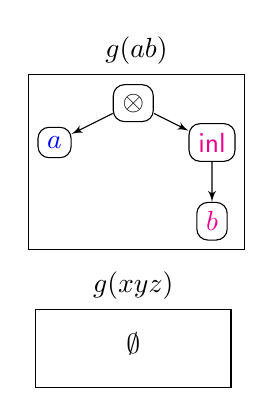
\begin{tikzpicture}[%opacity=0.5,
  treenode/.style = {shape=rectangle, rounded corners,
    draw, align=center,
    top color=white, bottom color=white!20},
    line/.style={draw, -latex'},
    edge from parent/.style={draw,-latex'},
    level 1/.style={sibling distance=20mm, level distance=0.5cm},
    level 2/.style={sibling distance=1cm, level distance=1cm},
    visible on=<3->
    ]
  \node[treenode] (tree) {$\otimes$}
    child { node[treenode] (a) {${\color{blue} a}$} }
    child { node[treenode] (b){${\color{magenta} \mathsf{inl}}$}
        child { node[treenode] (c) {${\color{magenta} b}$} }
      };
      \node[draw, fit=(tree)(a)(b)(c),
      label={[name=l] $g(ab)$}, visible on=<3->] {};
    \node[below=2.5cm of tree] (mt) {};
    \node[below=2.5cm of a] (mta) {};
    \node[below=2.5cm of b] (mtb) {};
    \node[below=-0.2cm of mt, visible on=<4->] (mtset) {$\emptyset$};
      \node[draw, fit=(mt)(mtset)(mta)(mtb),
      label={[name=l, visible on=<4->] $g(xyz)$}, visible on=<4->] {};
\end{tikzpicture}
  \end{minipage}%
  \begin{minipage}[t]{.6\textwidth}
    \[
      \onslide<5->{h = {\color{blue} a^{*}} \otimes {\color{magenta} a}}
    \]
  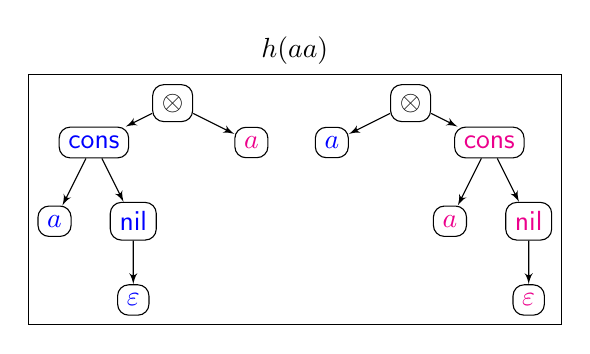
\begin{tikzpicture}[%opacity=0.5,
  treenode/.style = {shape=rectangle, rounded corners,
    draw, align=center,
    top color=white, bottom color=white!20},
    line/.style={draw, -latex'},
    edge from parent/.style={draw,-latex'},
    level 1/.style={sibling distance=2cm, level distance=0.5cm},
    level 2/.style={sibling distance=1cm, level distance=1cm},
    visible on=<6->
    ]

   \node[treenode] (tree) {$\otimes$}
   child { node[treenode] (a) {${\color{blue} \mathsf{cons}}$}
     child {node[treenode] (b) {${\color{blue} a}$}}
     child {node[treenode] (c) {${\color{blue} \mathsf{nil}}$}
       child {node[treenode] {${\color{blue} \varepsilon}$}}
     }
   }
   child {node[treenode] {${\color{magenta} a}$}}
    ;
   \node[treenode, right=2.5cm of tree] (tree2) {$\otimes$}
   child {node[treenode] {${\color{blue} a}$}}
   child { node[treenode] (x) {${\color{magenta} \mathsf{cons}}$}
     child {node[treenode] (y){${\color{magenta} a}$}}
     child {node[treenode] (z){${\color{magenta} \mathsf{nil}}$}
       child {node[treenode] (w){${\color{magenta} \varepsilon}$}}
     }
   }
    ;
      \node[draw, fit=(tree)(a)(b)(c)(x)(y)(z)(w),
      label={[name=l] $h(aa)$}, visible on=<6->] {};
\end{tikzpicture}
  \end{minipage}%
\end{frame}

\begin{frame}{Formal Languages and Equivalence}
  The \emph{formal language} for a grammar $g$ is the set of strings that match $g$

  \[
    L_{g} := \{ w \in \Sigma^{*} \mid g(w) \text{ nonempty}\}
  \]

  \onslide<2->{\textbf{(Chomsky, 1963)} Grammars $g$ and $h$ are\dots}
  \begin{itemize}
    \item<3-> \emph{weakly equivalent} if they generate the same language, $L_{g} = L_{h}$
    \item<4-> \emph{strongly equivalent} if there is a bijection between their sets of parse trees, $g \cong h$
  \end{itemize}

  \onslide<5->{i.e. $a$ and $a \oplus a$ are weakly, but not strongly, equivalent}
\end{frame}

\begin{frame}{Grammars and Their Automata}
  Correspondence between classes of grammars and the classes of machines that recognize them

  \begin{block}{Chomsky Hierarchy}
  \begin{center}
    \begin{tabular}{c c}
      \textbf{Grammar Class} & \textbf{Automata} \\
      Regular & Finite \\
      Context-free & Pushdown \\
      Context-sensitive & Linear-boundned \\
      Recursively-enumerable & Turing machine
    \end{tabular}
  \end{center}
  \end{block}
\end{frame}

\begin{frame}{A Finite Automaton}
  $g = a^{*} \otimes (b \oplus c)$

  \only<1-21>{\alert<21>{$\alert<7>{w} = \alert<8-10>{a} \alert<11-13>{a} \alert<14-16>{b}
    \only<18-19>{\otimes \alert{\varepsilon}}$} \quad \only<21>{ {\Large \color{cyan} \cmark}}}
  \only<22->{\alert<30>{$ w = \alert<23-25>{a} \alert<26-28>{b} \alert<29>{b}$}
     \quad \only<30>{ {\Large \color{magenta} \xmark}}}

  \onslide<3->{
  \begin{center}
  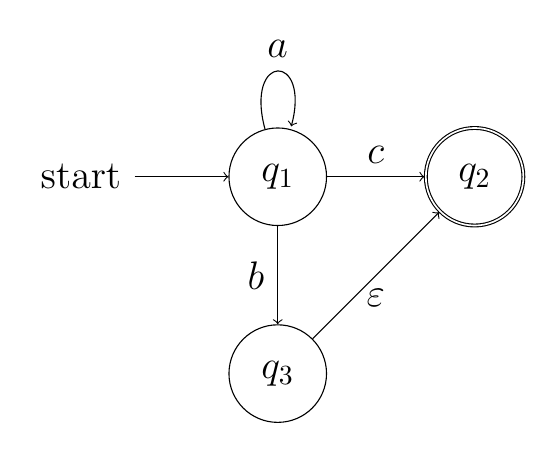
\begin{tikzpicture}[node distance = 25mm ]
    \Large
    \alert<4,8>{\node (0) {start};}
    \alert<4,8,10-11,13-14,23,25,26>{\node[state, right of=0] (1) {$q_{1}$};}
    \alert<5,20>{\node[state, right of=1, accepting] (2) {$q_{2}$};}
    \alert<16-17,28,29>{\node[state, below of=1] (3) {$q_{3}$};}

    \alert<15,27>{\draw[->] (1) edge[left] node{$b$} (3);}
    \draw[->] (1) edge[above] node{$c$} (2);
    \alert<9,12,24>{\draw[->] (1) edge[loop above] node{$a$} (1);}
    \alert<19>{\draw[->] (3) edge[below] node{$\varepsilon$} (2);}
    \alert<4,8>{\draw[->] (0) edge[above] node{} (1);}
  \end{tikzpicture}
  \end{center}}
\end{frame}



\section{Grammars as Types}

\begin{frame}{Why Types?}
  \textbf{(Firsov and Uustalu, 2015)} provide a verified context-free grammar parser, up to language equivalence

  \begin{itemize}
    \item<2-> Suggest an extension where parse trees are first-class objects
    \item<3-> Parse trees serve as proofs of language membership
    \item<4-> Under Curry-Howard, expect a corresponding type system
  \end{itemize}

  \onslide<5->{Grammar
  $g : \Sigma^{*} \to \Set$
  can be viewed as a functor}

  \begin{itemize}
    \item<6-> $\Sigma^{*}$ viewed as a discrete category
    \item<7-> Functors into $\Set$ --- presheaves --- have significant structure
    \item<8-> Presheaves model dependent type theory
    \item<9-> Design a type theory where grammars are the intended model
  \end{itemize}
\end{frame}

\begin{frame}{Grammars as Types}
  Types are \textbf{grammars}, and terms are \textbf{parse transformers}

  \begin{itemize}
    \item Take inspiration from linear logic and separation logic
    \item View the contetns of the string parsed as limited resources
  \end{itemize}

  \[
    x : c, y : a, z : t \vdash (x, y, z) : c \otimes a \otimes t
  \]
\end{frame}

\begin{frame}{Type Constructors}
\end{frame}

\begin{frame}{(Lack of) Structural Rules}
  Omit these structural rules that usually appear in intuitionistic logic

  \begin{mathpar}
    \onslide<2->{
    \only<2>{\inferrule*[Right=Weak]{\Delta \vdash M : g}{\Delta , x : A \vdash M : g}}
    \only<3->{\xcancel{\inferrule*[Right=Weak]{\Delta \vdash M : g}{\Delta , x : A \vdash M : g}}}}

    \and

    \onslide<4->{

    \only<4>{\inferrule*[Right=Contr]{\Delta , x : A , y : A \vdash  M : g}{\Delta , z : A \vdash
      M[ z / x , z / y ] : g}}
    \only<5->{\xcancel{\inferrule*[Right=Contr]{\Delta , x : A , y : A \vdash  M : g}{\Delta , z : A \vdash
      M[ z / x , z / y ] : g}}}
     }

    \\

    \onslide<6->{
    \only<6>{\inferrule*[Right=Exch]{\Delta , \Delta' \vdash M : g}{\Delta' , \Delta
      \vdash M : g}}
    \only<7->{\xcancel{\inferrule*[Right=Exch]{\Delta , \Delta' \vdash M : g}{\Delta' , \Delta
      \vdash M : g}}}}
  \end{mathpar}

  \onslide<8->{Entire context must be used, \emph{exactly once} and in order}

  \onslide<9->{Just like when reading a word}
\end{frame}
\begin{frame}{Defining a Parser}
  \onslide<1->{\alert<1>{Input string $w$}} \qquad \onslide<2->{\alert<2>{Grammar $g$}}

  \onslide<3->{
  \begin{block}{\alert<3>{Parser Term}}
    $$ \alert<4>{w : \Sigma^{*}} \vdash \alert<7>{\mathsf{parse}_{g}(w)} : \alert<5>{g} \oplus \alert<6>{\top} $$
  \end{block}}

  \onslide<8->{
  \begin{exampleblock}{Example}
    \begin{minipage}{.7\textwidth}
    \onslide<8->{\alert<8>{$g = a \otimes (b \oplus c)$}}

    \onslide<9->{\alert<9>{$w = ab$}}
    \onslide<10->{$\longrightarrow \mathsf{parse}_{g}(w) = {\color{cyan} \mathsf{inl}(p_{g})} : \alert<10>{g} \oplus \top$
    \quad {\LARGE \color{cyan} \cmark}}

    \onslide<11->{\alert<11>{$w = ad$}}
    \onslide<12->{$\longrightarrow \mathsf{parse}_{g}(w) = {\color{magenta} \mathsf{inr}(p_{\top})} : g \oplus \alert<12>{\top}$
    \quad {\LARGE \color{magenta} \xmark}}
    \end{minipage}%
    \begin{minipage}{.3\textwidth}
      \begin{center}
        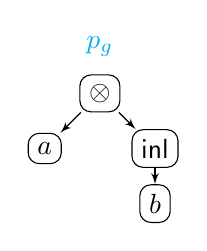
\begin{tikzpicture}[%opacity=0.5,
        treenode/.style = {shape=rectangle, rounded corners,
          draw, align=center,
          top color=white, bottom color=white!20},
          line/.style={draw, -latex'},
          edge from parent/.style={draw,-latex'},
          level 1/.style={sibling distance=20mm, level distance=1cm},
          level 2/.style={sibling distance=1cm, level distance=1cm},
          scale = 0.7, visible on=<10->
          ]
        \node[treenode] (tree) {$\otimes$}
          child {node[treenode] {$a$}}
          child {node[treenode] {$\mathsf{inl}$}
            child {node[treenode] {$b$}}}
          ;

        \node[above=0.1cm of tree, visible on=<10->] {$\color{cyan} p_{g}$};
        \end{tikzpicture}
      \end{center}
    \end{minipage}%
  \end{exampleblock}}



\end{frame}



% \begin{frame}{Kleene Star}
%   Take a least fixed-point operator $\mu$ as primitive

%   \onslide<2->{
%     Allows definition of recursive grammars
%   }

%   \onslide<3->{
%     \[
%       \inferrule{\Delta \vdash e : A[\mu x . A / x]}{\Delta \vdash \mathsf{cons}~e : \mu x . A}
%     \]
%   }
%   \onslide<4->{
%     \[
%       g^{*} := \mu {\color{YellowOrange} x} . ({\color{cyan}\varepsilon} \oplus ({\color{magenta} g} \otimes {\color{YellowOrange} x}))
%     \]
%   }
%   \onslide<5->{
%     Inductive data type with constructors,
%     \begin{itemize}
%       \item<5-> ${\color{cyan} \bullet} \vdash \mathsf{nil} : g^{*}$
%       \item<6->
%             ${\color{magenta} x : g}, {\color{YellowOrange} y : g^{*}} \vdash \mathsf{cons}(x , y) : g^{*}$
%     \end{itemize}
%   }
% \end{frame}

% \begin{frame}{Kleene Star Elimination}
%   Constructors
%   \[
%     {\color{cyan} \bullet \vdash \mathsf{nil} : g^{*}} \qquad {\color{magenta} x : g, y : g^{*} \vdash \mathsf{cons}(x , y) : g^{*}}
%   \]
%   \onslide<2->{
%   Eliminator
%   \[
%       \inferrule*[Right=$*$Elim]
%       {
%         {\color{cyan} \bullet \vdash p_{\varepsilon} : h} \\
%         {\color{magenta} x : g, y : h \vdash p_{*} : h}
%       }
%       {p : g^{*} \vdash \mathsf{fold}(p_{\varepsilon}, p_{*})(p) : h}
%     \]
%   }
%   \onslide<3->{
%     \begin{exampleblock}{Example}
%       \[
%       \inferrule
%       {
%         \onslide<4->{        \bullet \vdash \mathsf{nil : (ab)^{*}}} \\
%         \onslide<5->{x : abab, y : (ab)^{*} \vdash p_{*} : (ab)^{*}}
%       }
%       {p : (abab)^{*} \vdash \mathsf{fold}(\mathsf{nil},p_{*})(p) : (ab)^{*}}
%       \]
%     \end{exampleblock}
%   }
% \end{frame}


% \begin{frame}{Automata as Grammars}
%   $g = a^{*} \otimes (b \oplus c)$

%   \onslide<2-21>{\alert<21>{$\alert<7>{w} = \alert<8-10>{a} \otimes  \alert<11-13>{a} \otimes \alert<14-16>{b}
%     \only<18-19>{\otimes \alert{\varepsilon}}$} \quad \only<21>{ {\Large \color{cyan} \cmark}}}

%   \onslide<3->{
%   \begin{center}
%   \begin{minipage}{.5\textwidth}
%   \begin{tikzpicture}[node distance = 15mm, scale=0.4]
%     \alert<4,8>{\node (0) {start};}
%     \alert<4,8,10-11,13-14>{\node[state, right of=0] (1) {$q_{1}$};}
%     \alert<5,20>{\node[state, right of=1, accepting] (2) {$q_{2}$};}
%     \alert<16-17>{\node[state, below of=1] (3) {$q_{3}$};}

%     \alert<15>{\draw[->] (1) edge[left] node{$b$} (3);}
%     \draw[->] (1) edge[above] node{$c$} (2);
%     \alert<9,12>{\draw[->] (1) edge[loop above] node{$a$} (1);}
%     \alert<19>{\draw[->] (3) edge[below] node{$\varepsilon$} (2);}
%     \alert<4,8>{\draw[->] (0) edge[above] node{} (1);}
%   \end{tikzpicture}
%   \end{minipage}%
%   \begin{minipage}{.5\textwidth}
%     $$ \mathsf{Trace}(q_{1}, q_{2}) =$$
%     \begin{equation*}
%       \mu
%       \begin{pmatrix}
%         \alert<8,10,11,13,14>{g_{q_{1}}} := & \alert<9,12>{(a \otimes g_{q_{1}})} \\ & \oplus  ( c \otimes g_{q_{2}} ) \\ & \oplus \alert<15>{(b \otimes g_{q_{3}})} \\
%         \alert<20>{g_{q_{2}}} := & \alert<5,20>{\varepsilon} \\
%         \alert<16,17>{g_{q_{3}}} := & \alert<19>{g_{q_{2}}} \\
%       \end{pmatrix}. \alert<4>{\color<21>{cyan} g_{q_{1}}}
%     \end{equation*}
%   \end{minipage}
%   \end{center}}
% \end{frame}

% \begin{frame}{Accepting Traces of Automata}
%     \begin{minipage}{.5\textwidth}
%       \begin{tikzpicture}[node distance = 15mm, scale=0.4]
%         \node (0) {start};
%         \node[state, right of=0] (1) {$q_{1}$};
%         \node[state, right of=1, accepting] (2) {$q_{2}$};
%         \node[state, below of=1] (3) {$q_{3}$};

%         \draw[->] (1) edge[left] node{$b$} (3);
%         \draw[->] (1) edge[above] node{$c$} (2);
%         \draw[->] (1) edge[loop above] node{$a$} (1);
%         \draw[->] (3) edge[below] node{$\varepsilon$} (2);
%         \draw[->] (0) edge[above] node{} (1);
%       \end{tikzpicture}
%       \[ \mathsf{Trace}(\only<1>{q_{1}}\only<2->{\alert<2> {q_{2}}}, \only<1>{q_{2}}\only<2->{\alert<3>{q_{3}}}) \]
%       \begin{equation*}
%         \mu
%         \only<1>{
%         \begin{pmatrix}
%           g_{q_{1}} := & (a \otimes g_{q_{1}}) \\ & \oplus  ( c \otimes g_{q_{2}} ) \\ & \oplus (b \otimes g_{q_{3}}) \\
%           g_{q_{2}} := & \varepsilon \\
%           g_{q_{3}} := & g_{q_{2}} \\
%         \end{pmatrix}}\only<2->{
%         \begin{pmatrix}
%           g_{q_{1}} := & (a \otimes g_{q_{1}}) \\ & \oplus  ( c \otimes g_{q_{2}} ) \\ & \oplus (b \otimes g_{q_{3}}) \\
%           g_{q_{2}} := & \alert<4>{\bot} \\
%           g_{q_{3}} := & g_{q_{2}} \alert<3>{\oplus \varepsilon} \\
%         \end{pmatrix}
%         }. \only<1>{g_{q_{1}}}\only<2->{\alert<2>{g_{q_{2}}}}
%       \end{equation*}
%     \end{minipage}%
%     \begin{minipage}{.5\textwidth}
%       \onslide<5->{
%       \[
%         \mathsf{AccTrace} := \overline{\sum_{\alert<7>{q : Q}}} (\alert<8>{\mathsf{Trace}(q_{1}, q)}~\&~\alert<9>{\mathsf{acc}(q)})
%       \]
%       }
%       \begin{itemize}
%         \item<6-> An accepting trace is a triple\dots
%         \begin{itemize}
%           \item<7-> \alert<7>{An end state}
%           \item<8-> \alert<8>{A trace starting at the initial state}
%           \item<9-> \alert<9>{A proof that the end state is accepting}
%         \end{itemize}
%       \end{itemize}
%     \end{minipage}%
% \end{frame}


% \begin{frame}{Defining a Parser Term}
%   $D$ a DFA grammar

%   \[ w : \only<1>{\Sigma^{*}}\only<2->{\left( \bigoplus_{c \in \Sigma} c \right)^{*}} \vdash \mathsf{parse}_{D}(w) : \mathsf{AccTrace}_{D} \oplus \top \]

%   \onslide<3->{Define with Kleene star eliminator!}

%   \onslide<4->{
%     \[
%       A := \overline{\sum_{q : Q}} \mathsf{Trace}_{D}(q_{init}, q)
%     \]
%   \onslide<5->{
%   \[
%     \inferrule*[Right=$*$Elim]
%     {
%       \onslide<6->{\bullet \vdash p_{\varepsilon} : A} \\
%       \onslide<7->{x : A, y : \left( \bigoplus_{c : \Sigma} c \right) \vdash p_{*} : A}
%     }
%     {w : \left( \bigoplus_{c \in \Sigma} c \right)^{*} \vdash M : A}
%   \]}
%   }
%   \todoin{This slide is choppy and the bigoplus is confusing. Needs graphics}
% \end{frame}

% \begin{frame}{Results}
%   \begin{itemize}
%     \item<+-> We have a parser term for DFAs formalized in Agda
%     \item<+-> We want a parser for regular expressions
%     \item<+-> Prove that DFAs and regular expressions are equivalent to extend the DFA parser to a regular expression parser
%   \end{itemize}
% \end{frame}

% \begin{frame}{Regular Expressions and Finite Automata}
%   \begin{block}{Thompson's Construction (Formalized)}
%     For every regular expression $g$, we may construct an NFA $N_{g}$ that is isomorphic to $g$.
%   \end{block}

%   \onslide<2->{
%   \begin{block}{Determinization}
%     For every NFA $N$, there is a DFA $D$ that recognizes the same language
%   \end{block}}

%   \onslide<3->{Combine the above to realize a regular expression parser}
% \end{frame}

% \begin{frame}{More Expressive Language Classes}
%   \begin{itemize}
%     \item Finite automata correspond to regular expressions
%     \item<+-> Pushdown automata correspond to context free grammars
%     \item<+-> Can apply analogous constructions to achieve a verified parser for
%           (deterministic) context-free grammars
%     \item<+-> Restricted forms of context sensitivity
%   \end{itemize}
% \end{frame}

% \begin{frame}{Future Work}
%   Grammar theory has advanced since the 60s
%   \begin{itemize}
%     \item<2-> Interval parsing grammars \textbf{(Zhang et al., 2023)}
%     \item<3-> Binary data formats
%   \end{itemize}

%   \onslide<4->{There are other front end tasks}
%   \begin{itemize}
%     \item<5-> Semantic actions
%     \item<6-> Typechecking
%   \end{itemize}
% \end{frame}

% \begin{frame}{Related Work}
%   \begin{itemize}
%     \item<1-> CoStar \textbf{(Lasser et al., 2023)} gives a verified predictive
%           parser for non-left-recursive context free grammars (CFGs)
%     \item<2-> \textbf{(Danielsson, 2010)} gives a verified parser combinator library
%           in Agda
%       \begin{itemize}
%         \item<3-> Verified parser for general CFGs
%         \item<4-> \dots up to language equivalence
%         \item<5-> Mentions ``normalization by evaluation'' and proofs as
%               first-class objects
%       \end{itemize}
%   \end{itemize}
%   \todoin{Less text, expand on Danielsson}
% \end{frame}

\begin{frame}[standout]
  Questions?
\end{frame}

\end{document}
